\section{Om ordbogens tilblivelse -- pri la ekesto de la vortaro}
{\selectlanguage{danish}\itshape
de Jacob Nordfalk}

{\selectlanguage{english}
Inter 2007 kaj 2009 mia familio kaj mi lo\^gis en Nepalo, unu el la
landoj kun la plej malri\^caj lo\^gantaroj de la mondo (la\u{u} malneta
nacia produkto po lo\^ganto). Kvankam la esperantistoj tie elturni\^gas
diversmaniere, mi ofte pripensis \^cu ne eblus iel doni al ili
enspezojn: Pro la malaltaj salajroj kaj vivkostoj, nepalaj
esperantistoj povus fari laboron por Esperanto, kiu estus tro
longda\u{u}ra por fari libertempe en nia parto de la mondo. Mi sukcesis
kolekti monon por tiaj projektoj (interalie por fari la filmojn pri
Mejzi la Muso) inter esperantistoj de pli ri\^caj landoj.}

{\selectlanguage{english}
Tiam mi a\u{u}dis de Kim Henriksen pri la vortara projekto de Preben
Bagger: Li havis tre ellaboritan vortaron, sed nur kiel mane skribitan
manuskripton, kiun estus tro koste entajpi en Danio -- kaj venis la
ideo trovi nepalan esperantiston por fari tiun laboron. Mi telefonis al
Preben kaj proponis la ideon kaj ni interkonsentis elprovi \^cu la ideo
funkcios. }

{\selectlanguage{english}
Tiel interkonsentite, mi vizitis Preben Bagger somere 2009 kaj skanis
lian manuskripton. La literojn A-F li anta\u{u}e enkomputiligis, sed la
dosiero perdi\^gis -- li nenion plu havis enkomputile, nur surpapere.
Dum tago mi enskanis \^cion haveblan: 71 pa\^goj kun la literoj A-F kun
mane skribitaj korektoj, A-E sen korektoj (por transformi al
kruddokumento per optika signorekono), kaj G-T kiel mane skribita
manuskripto de 731 pa\^goj. }

{\centering\selectlanguage{english}

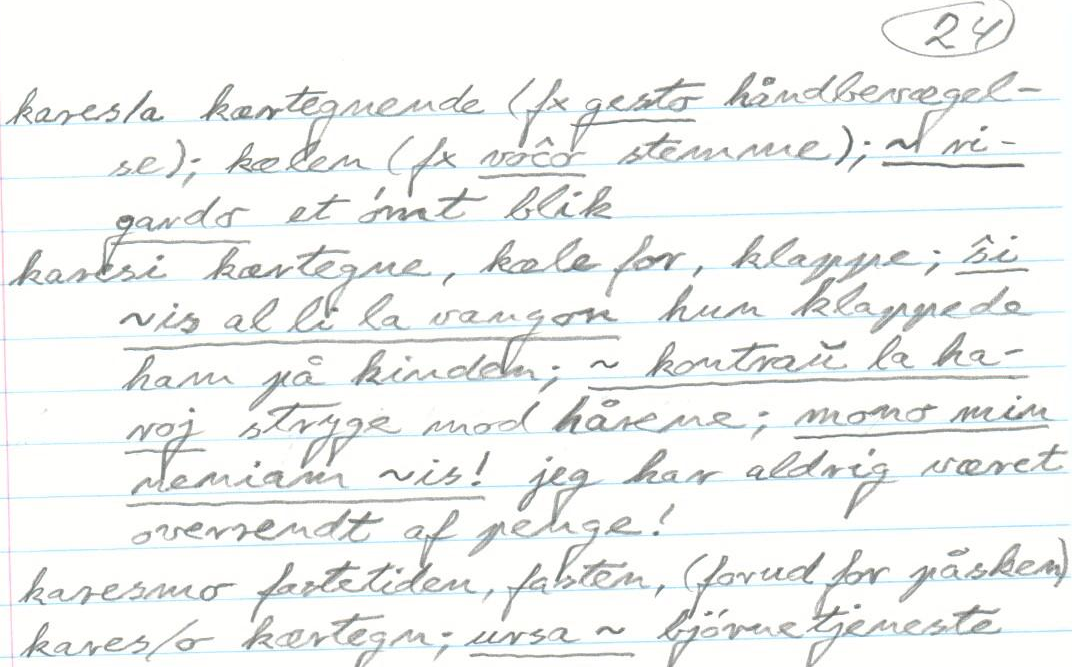
\includegraphics[width=8.749cm,height=5.443cm]{origino.png}
 
\par}

{\centering\selectlanguage{english}\itshape
Parto de unu el la 731 pa\^goj de la mane skribita manuskripto
\par}

{\selectlanguage{english}
Reveninte al Nepalo mi prezentis la manuskripton kaj la ideon al nepalaj
esperantistoj, kaj juna virino, Alinka Pokhrel, pretis preni la taskon,
kaj dum la sekva jaro \^si uzis pli ol 1500 laborhorojn por entajpi kaj
kontroli la 800 pa\^gojn, kontra\u{u} normala Nepala studenta salajro.
Danke al DEFA (Dana Esperanta Fervojista Asocio) ni ricevis malnovan
komputilon kun dana literumkontrolilo, kiu povis helpi \^sin literumi
preska\u{u} \^ciun danan vorton \^guste, kvankam \^si ne parolis la
danan: }

{\centering\selectlanguage{english}
\begin{minipage}{7.361cm}
{\selectlanguage{danish}
Pg. \foreignlanguage{danish}{24} }

{\selectlanguage{danish}
\foreignlanguage{danish}{kares/a k{\ae}rtegnende (fx
}\foreignlanguage{danish}{gesto}\foreignlanguage{danish}{
h{\aa}ndbev{\ae}gelse); k{\ae}len (fx
}\foreignlanguage{danish}{voc\^{}o}\foreignlanguage{danish}{ stemme);
}\foreignlanguage{danish}{\~{}rigardo}\foreignlanguage{danish}{ et
{\o}mt blik} }


\bigskip

{\selectlanguage{danish}
\foreignlanguage{danish}{karesi~~ k{\ae}rtegne, k{\ae}le for, klappe;
}\foreignlanguage{danish}{s\^{}i \~{}is al li~ la
vangon}\foreignlanguage{danish}{ hun klappeda ham p{\aa}~ kinden;
}\foreignlanguage{danish}{\~{} kontrau\^{} la
karoj}\foreignlanguage{danish}{ stryge mod h{\aa}rene;
}\foreignlanguage{danish}{mono min neniam
\~{}is!}\foreignlanguage{danish}{ jeg har aldrig v{\ae}ret overrendt af
penge!} }


\bigskip

{\selectlanguage{danish}
\foreignlanguage{danish}{karesmo~~~~~~~~~~ fastetiden,~ fasten, (forud
for p{\aa}sken)} }


\bigskip

{\selectlanguage{danish}
\foreignlanguage{danish}{kares/o k{\ae}rtegn;
}\foreignlanguage{danish}{ursa\~{}}\foreignlanguage{danish}{
bj{\o}rnetjenste} }

\end{minipage} 
\par}

{\centering\selectlanguage{english}\itshape
La sama parto, post entajpo de Alinka
\par}

{\selectlanguage{english}
\^Ciuj dosieroj de tiuj unuaj fazoj estas el\^suteblaj de la adreso:
\url{http://javabog.dk/esperanto/dana_vortaro_bagger/} . }

{\selectlanguage{english}
Dum 2010 mi ser\^cis kunlaborantojn kiuj volus helpi kontroli kaj
kompletigi la entajpitan manuskripton kaj trovis Jytte Sunek{\ae}r kaj
Peter Weide. Dum tri jaroj ni laboradis en nia libera tempo pri la
perfektigo de la manuskripto. Ni provis konservi la originalajn ideojn
kaj stilon de Preben, anka\u{u} en la literoj T, U, \u{U}, V kaj Z,
kiujn Peter Weide lerte ellaboris.}

{\selectlanguage{english}
Preben transdonis \^ciujn rajtojn pri la materialo al ni, .... kaj ni
nun \^satus pludoni tiun rajtojn al vi:}

\section{Permesilo -- copyright}
{\selectlanguage{danish}
Undertegnende Preben Bagger overdrager hermed Jacob Nordfalk samtlige
rettigheder over det til ham tidligere udleverede materiale til
ESPERANTO-DANSK ordbog, og jeg fraskriver mig hermed alle rettigheder
til det n{\ae}vnte materiale.}

{\selectlanguage{danish}
Vi, Peter Weide, Jytte Sunek{\ae}r og Jacob Nordfalk, tillader hermed
enhver digital og fysisk brug, {\ae}ndring og reproduktion af ordbogen,
s{\aa} l{\ae}nge der er en angivelse af kilden.}

{\selectlanguage{danish}
Vi har arbejdet med st{\o}rste omhu. Alligevel vil l{\ae}seren finde
fejl. Vi vil v{\ae}re taknemmelige, hvis man informerer os, s{\aa} vi
kan rette fejlene. Forslag til nye ord er selvf{\o}lgelig er ogs{\aa}
velkomne. Vi beder om at anvendelser i trykte ordb{\o}ger venter, til
denne udgave er udsolgt.}

{\selectlanguage{english}
\textit{Tiu \^ci verko estas komuna hava\^{\j}o; vi rajtas uzi la verkon
}\foreignlanguage{danish}{\textit{kia}}\textit{ \^gi estas, komerce
a\u{u} nekomerce, plibonigi, \^san\^gi, adapti. Kion ajn. La sola
kondi\^co estas ke vi menci}\textit{u}\textit{ la fonton.}}

{\selectlanguage{danish}
Ni laboris la\u{u}eble atenteme. Tamen eraroj trovi\^gos. Ni kun danko
akceptas informojn pri ili kaj la\u{u}eble rapide korektos ilin.
Memkompreneble anka\u{u} proponoj pri aldono de novaj vortoj estas
bonvenaj.}

{\selectlanguage{english}
Ni petas (ne postulas, sed petas) ke viaj uzoj ne rekte malgrandigu la
vendadon de tiu \^ci eldono, \^gis \^gi el\^cerpi\^gos.}


\bigskip

{\selectlanguage{english}
Jacob Nordfalk, Peter Weide kaj Jytte Sunek{\ae}r}

{\selectlanguage{english}
Valby, aprilo 2014.}


\bigskip


\bigskip


\bigskip


\bigskip

{\centering\selectlanguage{english}


\includegraphics[width=3.104cm,height=1.094cm]{permisilo.png}
 \newline

\par}

{\centering\selectlanguage{english}\itshape
\^Ci tiu verko estas disponebla la\u{u} la permesilo \newline
Krea Komuna\^{\j}o Atribuite 4.0 Tutmonda.\newline
Vi povas legi la tutan permesilon \^ce:\newline
 http://creativecommons.org/licenses/by/4.0/deed.eo
\par}
